\documentclass[10pt]{myNSF}

\usepackage{amssymb}
\usepackage{graphicx}
\usepackage{natbib}
\usepackage{url}
\usepackage{aastex_macros}
\usepackage{mypack}

\begin{document}

\title{An Ultrawideband Digital Signal Processing System for the Green
  Bank Telescope}
\maketitle

\section{Project Description}
\label{sec:project_description}

\subsection{Overview}
\label{sec:overview}

We propose to build a state-of-the-art ultra-wideband digital signal
processing (UWB-DSP) system for the Robert C.\ Byrd Green Bank
Telescope that will sample wide radio frequency (RF) bandwidths and
protect scientific data quality in the presence of strong radio
frequency interference (RFI).  The UWB-DSP system will ultimately be
deployed to directly sample the entire $0.7$--$4\; \GHz$ radio
frequency (RF) bandwidth of a new ultra-wideband radio receiver
(UWB-R) that is being developed in parallel for the GBT.  This
strategy will bypass the GBT's usual system of analog mixers and
filters that convert the RF signal to an intermediate frequency (IF).
The UWB-DSP system will also implement real-time radio frequency
interference (RFI) excision algorithms to identify and remove RFI in
the presence of astronomical signals.  The combination of real-time
RFI removal and high dynamic range digital sampling as close as
possible to the front-end receiver will make this complete UWB system
significantly more resistant to RFI than is currently possible with
existing technology on the GBT.  This is crucially important given the
experiences of a similar UWB system that has been deployed on the
Effelsberg Radio Telescope that was crippled by strong interference.

The primary science motivation for the UWB system is the direct
detection of low-frequency gravitational waves (GWs) via pulsar
timing.  The system will also allow for new, wideband spectral studies
of fast radio bursts (FRBs), magnetars, and other radio transients, as
well as faster surveys of regions rich in molecular lines at these
frequencies (e.g. H{\sc II} radio recombination lines and complex
chemical species).  

This project will be broken into two phases, \emph{the first of which
  will be supported by this ATI:}
\begin{itemize}
\item{\textbf{Phase {\sc I}:} Research and develop the next generation
    of digital signal processing hardware, firmware, data transmission
    protocols, and RFI removal techniques.}
\item{\textbf{Phase {\sc II}:} Integrate the technologies and
    techniques developed in phase one into the UWB-R, which will then
    be deployed as a complete, facility instrument.}
\end{itemize}

The UWB-DSP system will use fast, high dynamic range analog to
digital converters, powerful field programmable gate arrays
(FPGAs), innovative RFI excision techniques not in use at any
other observatories, and pioneering methods for handling very high
data rates using 100-gigabit Ethernet (GbE) protocols.  These will
complement the UWBR, which will deliver a combination of wider
instantaneous bandwidth and lower system noise temperature than was
possible with previous generation technology.  Our project will thus
pair advanced digital and analog technologies for the world's largest
single-dish radio telescope to enable transformative scientific
advances in cutting edge fields of astronomy and astrophysics.

The UWB system will be open for use by the full astronomical community
via NSF-funded open skies programs.  This project will also serve as a
pilot program for upgrades to the GBT's existing receivers and IF
system.  All of the hardware design, firmware, and software developed
through our efforts will be made publicly available for use at other
observatories, and will be directly relevant for possible future
telescopes such as the Next Generation Very Large Array (ngVLA) and
Square Kilometer Array (SKA).  We will also leverage GBO's leadership
in the NSF INCLUDES program to broaden participation in digital
engineering and radio astronomy via an annual summer camp for
undergraduate students.  During this camp students will directly
participate in the RFI excision project by creating training data sets
for machine learning algorithms.  The students will also be exposed to
a wide range of engineering and scientific disciplines that contribute
to the success of GBO, and will receive interventions that will
increase retention in STEM fields.  An additional full-time summer
undergraduate student will work directly with experts at GBO and the
University of California-Berkeley on digital engineering for the
UWB-DSP project.  This will create a pipeline of students for GBO's
successful summer student programs (including our NSF-funded REU
program), alumni of which have already contributed to the RFI excision
project.  The UWB-DSP project will thus have an extremely broad impact
on the wider scientific community and the next generation of STEM
professionals.

\subsection{Intellectual Merit}
\label{sec:IM}

\subsubsection{Motivation}
\label{sec:motivation}

Our objective is to enable a diverse range of high-impact astronomical
science benefiting from ultra-wide bandwidths at radio frequencies,
particularly the study of pulsars and transients, and of rich
molecular line regions.  We will also develop technical solutions for
sharing the radio spectrum with civil and commercial users.  New DSP
hardware makes both goals feasible and especially timely.  We describe
the science and technical motivations for this project in more detail
below.

\subsubsubsection{Scientific Motivation}
\label{sec:science_motivation}

\alanheading{The Low-Frequency GW Universe} The primary science driver
of the UWB-DSP system is the direct detection of nanohertz frequency
GWs via pulsar timing, which is the focus of the NSF-supported North
American Nanohertz Observatory for Gravitational Waves Physics
Frontier Center (NANOGrav PFC; \cite{mcl13}).  At these GW frequencies
the dominant source class is expected to be supermassive binary black
holes (SMBBH) in the early stages of inspiral at the centers of
galaxies; exotic sources of GWs such as cosmic strings may also emit
in the $\nHz$-regime.  The NANOGrav PFC and similar experiments are
highly complementary to ground- and space-based laser interferometers
that probe higher GW frequencies, and cosmic microwave background
experiments that probe lower frequencies (see Figure
\ref{fig:gw_spectrum}).  The NANOGrav PFC is on-track to detect a
stochastic GW background within the next 3--5 years \citep{tve+15},
and is already placing important constraints on the amplitude of this
background that informs models of SMBBH evolution and coupling to the
surrounding galactic environments \citep{abb+16,abb+18}.  The
detection of individual continuous wave sources is expected to follow
in the coming decade, which will enable multi-messenger studies of
SMBBH systems.  The NANOGrav PFC also places the most stringent
existing limits on the energy density of cosmic strings
\citep{abb+18}.

\begin{figure}
  \centering
  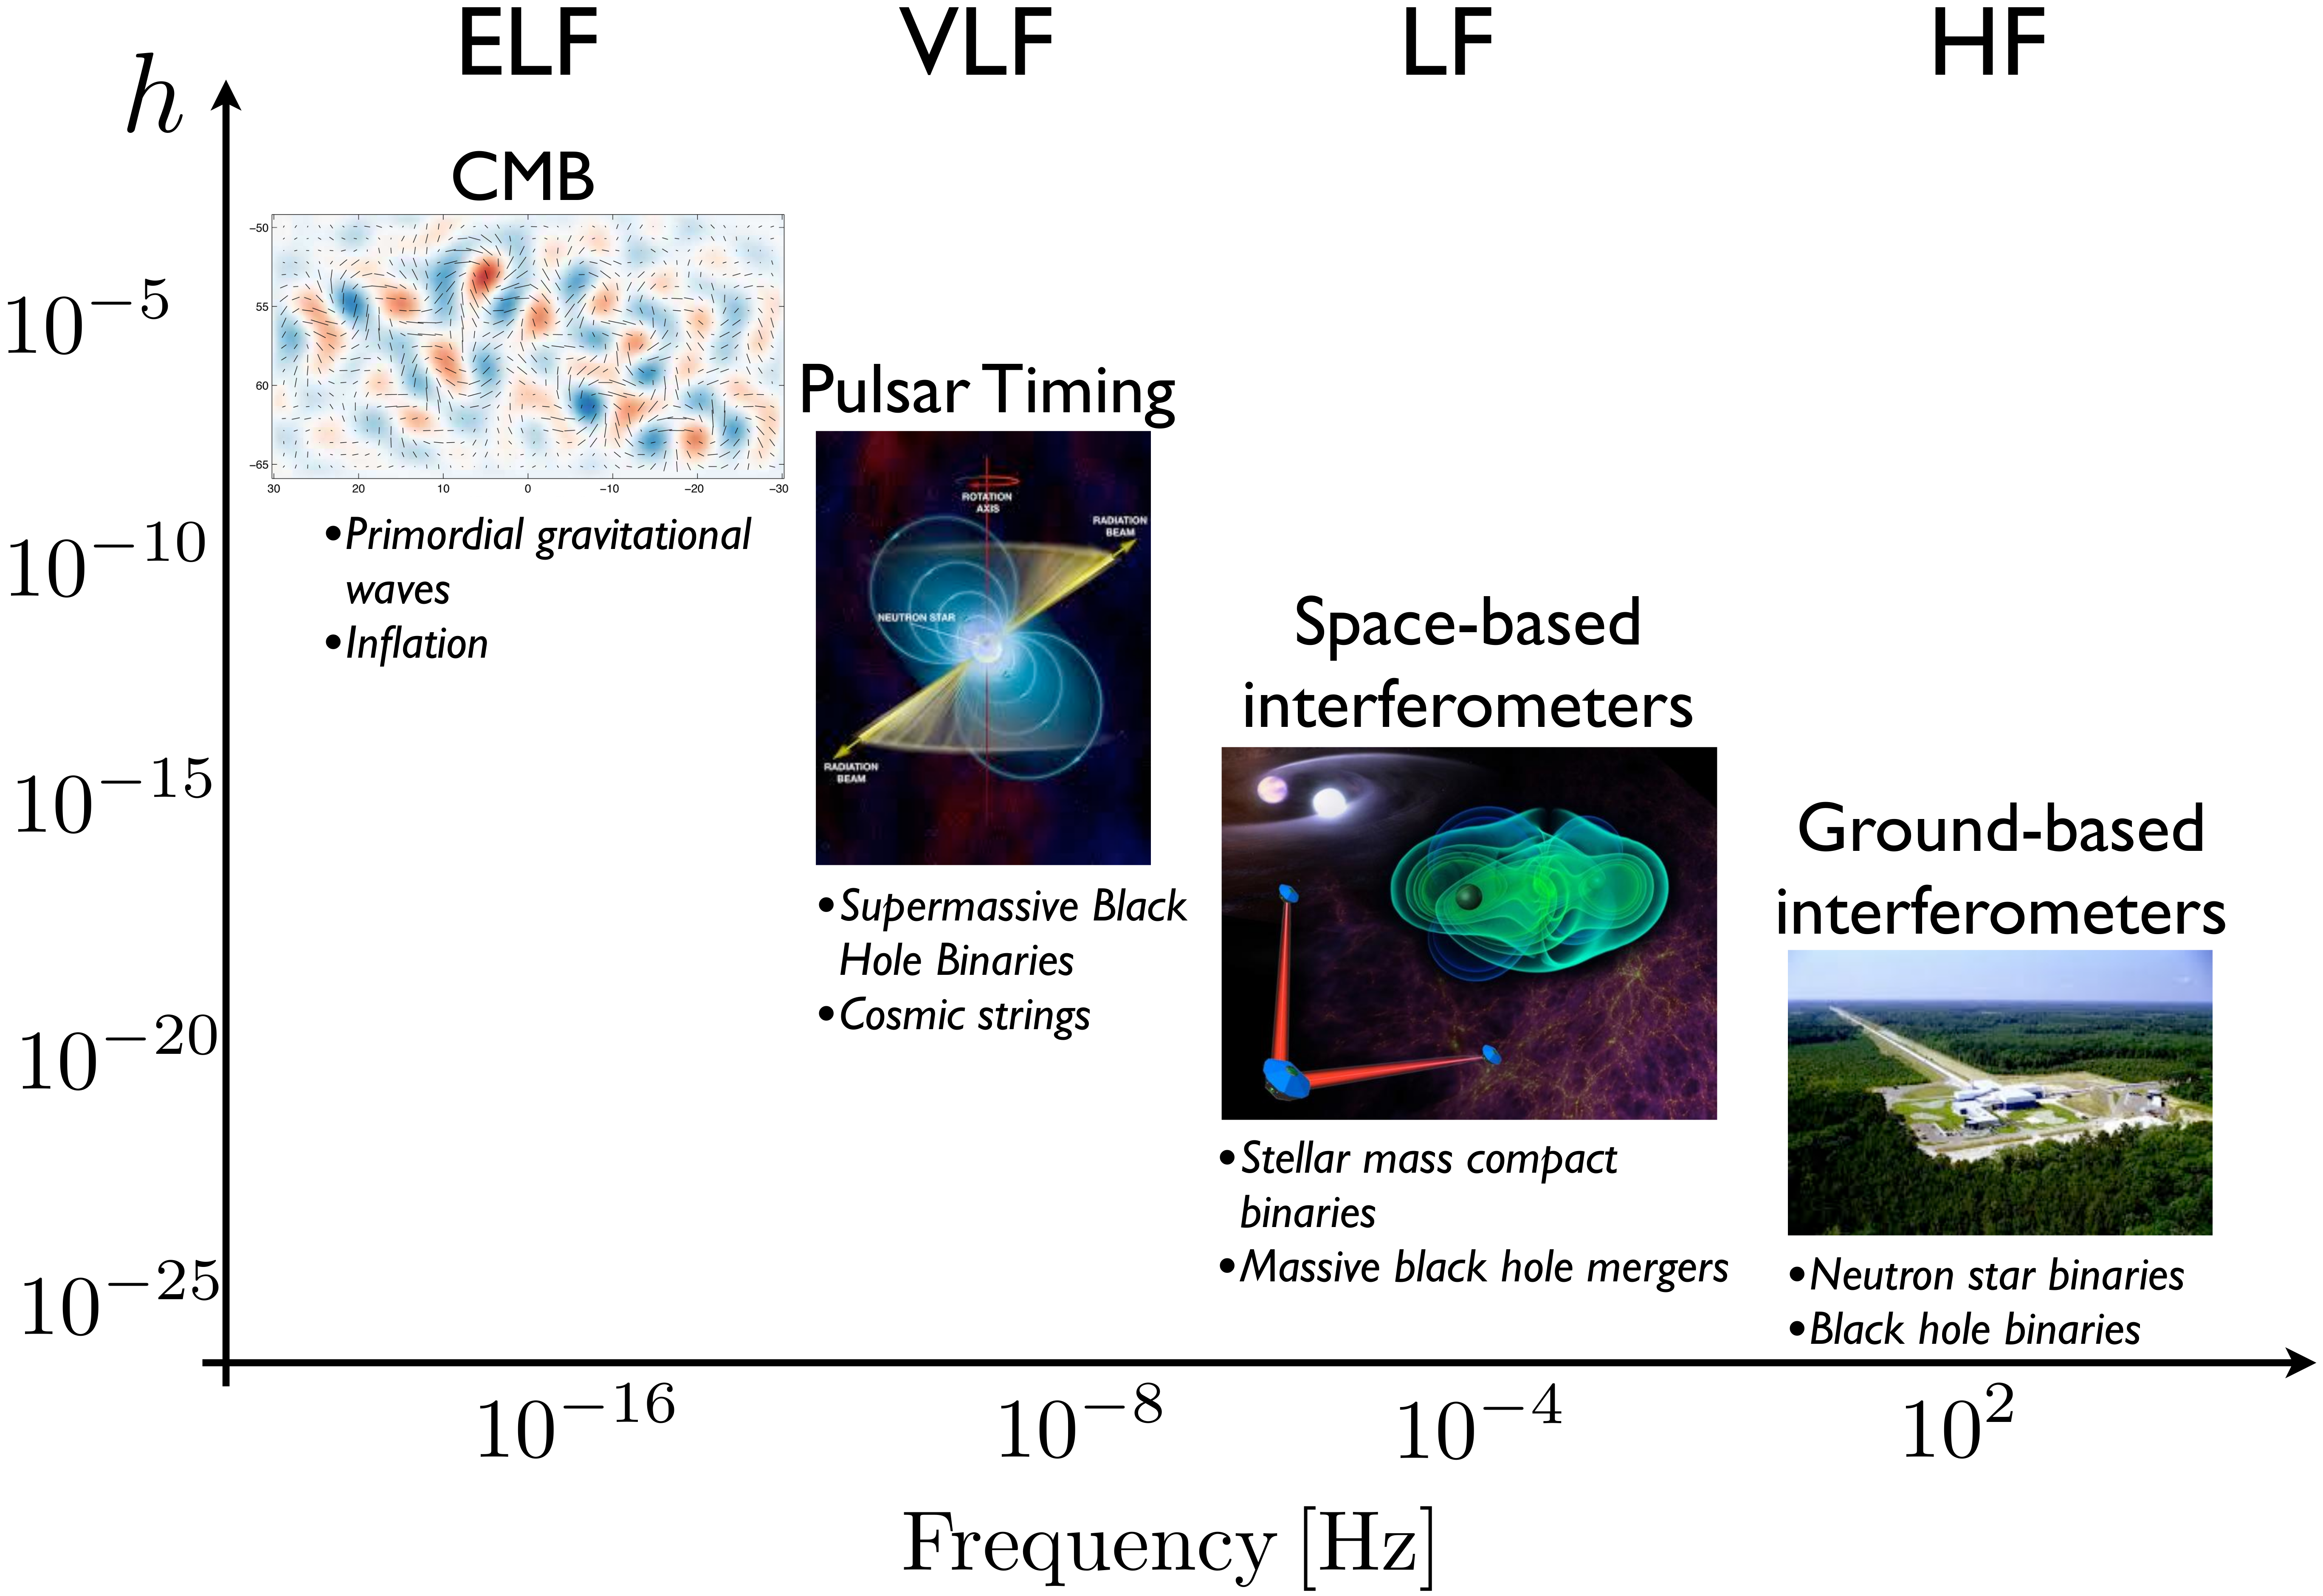
\includegraphics[width=0.65\textwidth]{gw_spectrum.png}
  \caption{Like the electromagnetic spectrum, the GW spectrum spans
    orders of magnitude and a variety of source-classes that can only
    be fully studied using complementary techniques.  PTAs probe lower
    GW frequencies than ground- and space-based interferometers, and
    higher frequencies than cosmic microwave background polarization
    experiments (Figure courtesy of the NANOGrav
    PFC). \label{fig:gw_spectrum}}
\end{figure}

The NANOGrav PFC uses the GBT and the William E. Gordon telescope at
the Arecibo Observatory (AO) to observe a pulsar timing array (PTA) of
millisecond pulsars (MSPs) distributed across the sky.  The extremely
high rotational stability of MSPs allows them to be used as clocks
whose ``ticks'' are pulse times of arrival (TOAs) that can be
accurately measured \emph{and predicted} with accuracies of $\lesssim
100\; \ns$ over time scales of decades.  The influence of GWs at the
Earth will cause a $10$--$100\; \ns$ deviation in the TOAs because of
the changing path-length between the observer and the pulsars.  The
quadripolar nature of GWs will specifically cause a quadripolar
angular correlation between pulsars distributed across the sky, which
makes it possible to distinguish between GWs and other sources of TOA
deviations (e.g. uncorrelated effects on individual pulsars, or
observatory clock errors or Solar System effects that will have a
monopolar and dipolar angular correlation, respectively; \cite{hd83}).
This process of pulsar timing demands a complete characterization of
the MSPs themselves, including their rotational, astrometric, and
binary properties.  Thus, other high-impact science emerges from this
project, such as pulsar mass measurements \citep{epe+16}, tests of
general relativity \citep{zsd+15}, and novel constraints on Solar
system planetary ephemerides \citep{abb+18}.

One of the most important steps in obtaining TOAs with the required
accuracy is measuring and correcting for the effects of the ionized
interstellar medium (ISM) on pulsar signals.  One of these effects is
a dispersive delay given by
\begin{equation}
  \Delta t_{\rm DM} = \frac{k_{\rm DM} \, \DM(t,f)}{f^{-2}}
\end{equation}
where $k_{\rm DM}$ is a physical constant, $f$ is the radio frequency,
and $\DM(t,f)$ is the dispersion measure, i.e. column density of free
electrons between the pulsar and the Earth \citep[e.g.][]{lk12}.  We
emphasize that \DM\ is both time and frequency dependent
\citep{css16}, and thus represents a noise term \emph{that must be
  measured at each observing epoch with a fractional precision of
  $\sim 10^{-5}$}.

The NANOGrav PFC currently employees a two-receiver strategy at the
GBT to precisely measure DM, observing from $0.72$--$0.92\; \GHz$ and
$1.1$--$1.9\; \GHz$.  This approach is sub-optimal for several
reasons.  First, it effectively doubles the observing time needed to
obtain a single TOA.  Second, for operational reasons these
observations are typically scheduled with a separation of a few days,
making it impossible to resolve DM variations on shorter timescales.
\emph{The UWB system will double the observational efficiency of
  high-precision pulsar timing programs while improving measurements
  of DM.  When coupled with higher pulsar signal-to-noise from the
  wider instantaneous bandwidth, the NANOGrav PFC's sensitivity to GWs
  will increase at twice the rate as without an UWB system}.  This in
turn will effectively double the volume over which the NANOGrav PFC is
sensitive to individual SMBBHs---analogous to the improvement between
the first phase of the Laser Interferometric Observatory for
Gravitational Waves (LIGO) and Advanced LIGO.

\alanheading{Radio Transients} Wide instantaneous bandwidth is
essential for characterizing the spectro-temporal behavior of highly
variable radio transients.  One such population are fast radio bursts
--- millisecond duration radio-frequency pulses that originate in
distant galaxies \citep{lbm+07,tsb+13}.  Their physical origin is one
of the most pressing mysteries in astronomy and will be a major area
of research in the coming decade.  To-date, only one FRB has been
observed to repeat (FRB 121102; \cite{sch+14,ssh+16a}), a fact which
has enabled the only precise interferometric localization of an FRB to
a host galaxy \citep{clw+17,tbc+17}, as well as long-duration study of
the changing characteristics of the bursts (e.g. DM, Faraday rotation
measure (RM), and burst morphology; \cite{msh+18}).  With telescopes
like the Australian SKA Pathfinder and the Canadian HI Intensity
Mapping Experiment poised to discover dozens (if not hundreds) of new
FRBs \citep{smb+18,chime18}, more repeaters are sure to follow.

FRB 121102 exhibits dramatic burst-to-burst spectro-temporal variation
including a) a highly variable power-law spectral index; b)
non-power-law spectral shapes including band-limited bursts; c)
changing peak frequency; d) changing burst morphology; and e) distinct
sub-bursts that drift towards lower peak frequencies with time in the
larger burst envelope \citep{ssh+16b}.  These features may be
intrinsic, extrinsic, or both --- the sub-burst structure in
particular may be a sign of plasma lenses in the local environment of
FRB121102 \citep{cwh+17,myc+18}.  There is also some evidence for
secular changes in DM and RM \citep{msh+18,gsp+18}.  All bursts thus
far have been detected between $\sim 1$--$8\; \GHz$ despite
significant observing campaigns at lower and higher frequencies.

Any theory regarding the nature of FBR 121102 (and presumably at least
some class of FRBs more generally) must explain these wideband
properties, so they serve as a powerful diagnostic tool for
understanding FRBs' physical origins.  However, most burst detections
are limited by the bandwidth of the receiver, so the only way thus far
to investigate the behavior of FRB 121102 over ultra-wide bandwidths
has been through simultaneous observations using multiple telescopes.
This is obviously logistically complicated and sub-optimal.  Our new
UWB system will enable spectro-temporal studies of FRB 121102 and
future repeating FRBs, answering critical questions such as a) does
the characteristic bandwidth of bursts change with frequency, and if
so, with what form? b) do band-limited bursts appear simultaneously in
widely separated sub-bands? c) do sub-bursts cluster in frequency and
time, or can the peak frequency change on burst-to-burst timescales?
d) what is the burst morphology over ultra-wide bandwidths? e) is the
apparent $\sim 1\; \GHz$ lower limit real or an artifact of
under-sampling at lower frequencies? and f) does DM vary as a function
of frequency in broad-band bursts?  The answers to these questions can
then be quantitatively compared with physical models for FRB emission,
such as the aforementioned plasma-lensing model.

A second class of variables are radio magnetars --- neutron stars
whose emission is powered by the decay of extremely strong magnetic
fields.  To-date only four radio magnetars have been discovered out of
a larger population of 29\footnote{See
  \url{http://www.physics.mcgill.ca/~pulsar/magnetar/main.html} for an
  up-to-date list.} magnetars that emit X-rays and gamma-rays
\citep{crh+06,crh+07,lbb+10,efk+13}.  Their sporadic emission and
variable power-law spectral index, polarization fraction and position
angle, and burst morphology stand in stark contrast to
rotation-powered radio pulsars \citep[e.g.][]{crp+07}, and the details
of the radio emission mechanism remains a mystery.  As with FRB
121102, spectro-temporal studies have been limited by the relatively
small bandwidth provided by most receivers.  Interestingly, there may
be a connection between magnetars and FRBs.  A young, powerful
magnetar is one of the leading candidates for the source of FRB 121102
\citep[e.g.][]{mm18}, and the extremely high RM observed in FRB 121102
has only one known analog: the radio magnetar near the center of the
Milky Way \citep{efk+13}.  Thus, studies of magnetars may improve our
understanding of FRBs, and vice versa.  The UWB-DSP system will thus
be a powerful tool for expanding our knowledge of radio transients.

\alanheading{Molecular Line Surveys} \textbf{TODO}

\subsubsubsection{Technical Motivation}
\label{sec:technical_motivation}

The ultra-wide bandwidth observations needed to realize the above
scientific potential come with a number of technical challenges.  The
primary technical motivation for the UWB-DSP system is also one of the
most pressing: the ability to \emph{share the spectrum} with man-made
transmitters while producing scientifically usable data at frequencies
where there is significant, strong RFI.  GBO's location at the center
of the 13,0000 square-mile National Radio Quiet Zone and smaller West
Virginia Radio Astronomy Zone gives it unique interference protection,
but many sources of RFI, such as satellite transmitters, are
unavoidable (for more information on these interference protection
zones see Facilities, Equipment, and Other Resources).  The ability to
effectively coexist with other spectrum users is made all the more
important by the expanding presence of wireless devices in our lives
(such as the inevitable pervasiveness of self-driving cars relying on
RADAR or similar active-RF methods for guidance), as well as the
increasing sensitivity and bandwidth of astronomy receiver systems
(and thus the total number of RFI detections per-second).

We broadly classify techniques for sharing the spectrum into RFI
resistance (i.e., a high linear dynamic range in every analog and
digital component of the signal processing chain) and RFI excision
(i.e. removal of RFI at the lowest-possible level of data to improve
data quality).  We note that GBO is taking extreme care to ensure that
the front-end UWBR is sufficiently resistant to RFI as part of a
separate research and development effort, so here we concern ourselves
only with the UWB-DSP system.

\alanheading{RFI Resistance} The GBT currently uses the Versatile
Green Bank Astronomical Spectrometer (VEGAS, developed in part with
support from NSF award AST-1006509) as its primary digital back-end
system.  VEGAS uses eight spectrometer banks each consisting of $2
\times 3\; \mathrm{Gsps}$ 8-bit ADCs (one for each polarization
channel) paired with a high-performance computer (HPC) equipped with
an nVidia GTX 780 graphical processing unit (GPU).  A relatively
straightforward expansion of the HPC system will be sufficient to
process the full bandwidth provided by the UWBR for pulsar and FRB
observations, but this approach comes with significant drawbacks.
Most notably, VEGAS makes use of the GBTs IF system before digital
sampling, which will expose the UWB system to potential saturation of
numerous components including the RF-over-fiber transceivers, two
additional frequency mixers and bandpass filters, and the VEGAS 8-bit
ADCs.  These concerns are not esoteric ---- in recent months GBO staff
have become aware of total power instabilities that are present in the
$1$--$2\; \GHz$ band.  These instabilities are seen in a variety of
digital back-end systems, including VEGAS, and have been traced to the
growing use of automatic dependent surveillance-broadcast (ADS-B)
technology\footnote{ADS-B is used for air traffic control as part of
  the Next Generation Air Transportation System and is intended to
  replace secondary surveillance RADAR.  It will be required on all
  aircraft operating in the United States by 2020.  See
  \url{https://www.faa.gov/nextgen/programs/adsb/}} transmitting at
$1.09\; \GHz$; the instability itself has been isolated to non-linear
response of analog components between the RF-over-fiber transcievers
and second frequency mixer.  The UWB system will be exposed to an even
worse RFI environment that includes cellular communication towers,
digital television transmitters, Global Positioning System satellites,
airport radar and aircraft positioning systems, Iridium communication
satellites, and Sirius XM Satellite Radio.  \emph{We thus have
  empirical evidence that illustrates the need to minimize the analog
  components in the UWB signal path and to digitally sample with
  sufficient dynamic range to maintain linearity across $0.7$--$4\;
  \GHz$}.

The UWB-DSP system will accomplish this goal by completely bypassing
the existing GBT IF system, sampling at RF with a minimum of 12-bits
per polarization channel.  This will also provide better spectral
baseline stability.

\alanheading{RFI Excision} GBO has been actively testing several
techniques for automated RFI detection and excision.  These include
the use of median absolute deviation of complex voltage samples,
spectral kurtosis, robust recursive power estimation, and a new
project using machine learning (ML) algorithms.  However, the
limitations of our existing ROACH2-based DSP hardware prevents us from
fully implementing, testing, and deploying these RFI excision
techniques.  Specifically, this previous generation hardware has a
comparatively low number of on-board resources such as block random
access memory (BRAM), DSP cores, and logic cells, as well as low
bandwidth I/O transceivers.  We have also struggled to meet timing
closure using the Virtex-6 technology for complex firmware designs.

Luckily, new developments in FPGAs and associated tool flows
fundamentally change the paradigm for realizing sophisticated RFI
excision techniques.  New FPGAs have improved memory capacity, logic
density, and I/O bandwidth.  Improvements in development tools make it
easier to achieve timing closure and to build complex programs,
leading to faster prototyping, testing, and deployment.  \emph{Our
  development of an UWB-DSP system is perfectly timed to take
  advantage of these new technologies to integrate real-time RFI
  excision into standard data-processing pipelines.}

\alanheading{Next Generation Hardware} In only the last few months,
industry leaders have started to offer a number of exciting and
powerful new ADCs and FPGAs.  We have identified two products in
particular that improve by factors of several over the generation of
hardware used in VEGAS.
\begin{enumerate}
\item{The \textbf{Analog Devices AD9213} is a $10.25\; \mathrm{Gsps}$
    12-bit ADC which is representative of the upcoming generation of
    high-speed ADCs.  The AD9213 is faster, more precise, and has
    lower noise than our current EV8AQ160 (see Table
    \ref{table:adcs}).  One large driver behind the lower spur-free
    dynamic range is the improved manufacturer-provided calibration
    techniques for the suppression of multi-core interleaved suprs
    that are inherent in pipelined ADC technologies (considerable work
    was required by GBO and CASPER to properly calibrate our existing
    ADCs).  \emph{The fast sampling rate, bit-depth, and $6\; \GHz$
      full-power bandwidth provided by the AD9213 will allow us to
      directly sample the UWB-R at RF.}}
\item{We are in need of a successor to the CASPER ROACH2 boards that
    were the core of our previous generation DSP systems.  The Xilinx
    Virtex UltraScale+ FPGA VCU118 evaluation kit is a promising
    platform.  The VCU118's FGPA has significantly more resources than
    the ROACH2 (allowing larger, more computationally intense
    designs), significantly smaller feature size (simplifying timing
    closuer), and significantly faster transceivers (allowing higher
    I/O bandwidth).  Table \ref{table:fpgas} provides a side-by-side
    comparison.  \emph{These new FPGAs will provide the critical
      resources needed to implement real-time RFI excision over very
      wide bandwidths alongside standard DSP procedures
      (e.g. channelization).}}
\end{enumerate}
This ATI proposal is thus perfectly timed to take advantage of
cutting-edge technology in the service of our scientific and technical
goals.

\begin{table}[h]
  \centering
  \caption{Comparison of ADC Standards \label{table:adcs}}
  \begin{tabular}{|l|c|c|}
    \hline
    Feature/Spec & E2V EV8AQ160 & AD AD9213 \\
    \hline
    Max. Sampliing Rate & $5\; \GHz$ & $10.25\; \GHz$ \\
    Bit-depth & 8 & 12 \\
    Spur-free Dynamic Range (@max. rate) & $56\; \mathrm{dBc}$ & $68\; \mathrm{dBc}$ \\
    Power Consumption (@max. rate) & $4.2\; \mathrm{W}$ & $5.1\; \mathrm{W}$ \\
    Effective Number of Bits (@ max. rate) & 7.1 & 8.7 \\
    \hline
  \end{tabular}
\end{table}

\begin{table}[h]
  \centering
  \caption{Comparison of ROACH2 and VCU118 \label{table:fpgas}}
  \begin{tabular}{|l|c|c|}
    \hline
    Resource & ROACH2 & VCU118 \\
    \hline
    FPGA System Logic Cells & 476K & 2586K \\
    FPGA DSP Slice & 2016 & 6840 \\
    FPGA BRAM & $38\; \mathrm{Mb}$ & $6840\; \mathrm{Mb}$ \\
    Board DDR4 & $2\; \mathrm{GB}$ & $8\; \mathrm{GB}$ \\
    High-Speed Ethernet & $8 \times 10\mathrm{-GbE}$ & $3 \times 100\mathrm{-GbE}$ \\
    FPGA Silicon Feature Size & $40\; \nm$ & $16\; \nm$ \\
    Expansion Bus & $2 \times \mathrm{ZDOK}$ & $1 \times \mathrm{FMC}$, $1 \times \mathrm{FMC}+$ \\
    Max FPGA transceiver speed & $6.6\; \mathrm{Gbps}$ & $32.75\; \mathrm{Gbps}$ \\
    \hline
  \end{tabular}
\end{table}

\subsubsection{Innovation}
\label{sec:innovation}

Our use of emerging technology in the UWB-DSP system means that there
is no turn-key solution available.  Instead, we will develop new
procedures for integrating various hardware components, as well as new
firmware, data transmission methods, and network topologies for very
high data rates.  We will also begin implement and test various RFI
excision strategies.  To the extent possible we will use modular
designs that abstract away lower-level components.  This will make it
easier to rapidly take advantage of future technologies as they
emerge, so that the impact of our efforts will last much longer than a
single generation or specific architecture.  All of our work will be
conducted in an open and collaborative framework for use by other
observatories and interested parties.  In the following sections we
detail the specific tasks that will be accomplished as part of Phase
{\sc I} of the UWB-DSP project that is supported by this ATI.

\subsubsubsection{Integrating New ADCs and FPGA Boards}
\label{sec:adc_fpga}

One benefit of the ROACH2 over the VCU118 is that the ROACH2 was
specifically designed by a radio astronomy research and
instrumentation organization with radio astronomy applications in
mind, whereas the VCU118 is a development board developed by Xilinx
whose purpose is to exhibit the full range of the possibilities
created by the Virtex UltraScale+ series chips. Functionally, the one
area of the boards where this discrepancy is made obvious is the
high-speed transceivers --- on the ROACH2 all of the transceivers are
connected to expansion bus connectors, whereas many transceivers on
the VCU118 are connected to ``exhibition'' technologies (PCIe, Samtec
FireFly) that we do not intend to use on our deployed
VCU118s. Nevertheless, the overall ``useable'' I/O bandwidth of the
VCU118 far exceeds that of the ROACH2.

We will experiment with two techniques for direct RF sampling over the
bandwidth of the UWB-R.  The first, most straightforward approach is
to clock the ADCs near their maximum rate, digitizing the entire
$0.7$--$4\; \GHz$ with one sampler.  This would simplify downstream
processing by avoiding the need to stitch together different
sub-bands, but does come at the cost of a lower effective number of
bits (ENOB; the pre-release specifications for the AD9213 quote 8.7
bits at the maximum sampling rate of $10.25\; \mathrm{Gsps}$).  The
second approach would use a simple signal-splitter to produce two or
three copies of the UWB-R signal, which would each be sent to a
seperate pair of ADCs (one for each polarization) clocked at slower
speeds.  The first copy would be low-pass filtered and sampled at base
band (i.e. the first Nyquist zone), while higher frequencies would be
bandpass filtered to prevent alisasing and sampled in higher Nyquist
zones.  This would still bypass the existing GBT IF system and would
have the advantage of offering a higher ENOB, at the expense of
additional processing steps.  We will determine if the better dynamic
range in the second approach is needed and select the most appropriate
path forward for the final, production system.

\subsubsubsection{Firmware Development}
\label{sec:firmware}

\emph{We will develop firmware designs for the next-generation
  hardware and communication protocols deployed in the UWB-DSP system.
  These designs will be shared widely with the scientific and
  engineering communities.}

In light of the variety of new hardware that we will use in the
UWB-DSP system, a variety of new firmware ``blocks'' (sets of
low-level FPGA code abstracted to a higher level for easier use by
firmware system designers) will need to be developed for interfacing
with various FPGA-facing peripherals as well as for executing advanced
DSP techniques.  In addition, new firmware tools may need to be
developed to allow our CASPER-based designs to take advantage of the
totality of hardware advancements that are provided by Xilinx
UltraScale+ and later technologies. Much of this new firmware
development can be broken into functional blocks within Xilinx's
Embedded Developer's Kit (EDK) architecture. Basic EDK blocks are
primarily dedicated to data processing with no use of peripheral
components (e.g. BRAM, transceivers, Microblaze access, etc.), whereas
CASPER EDK blocks interface with peripherals. Many of the CASPER EDK
blocks exist for earlier generations of hardware, but considerable
work is required to prepare them for the newest generations. A
discussion of prospective developments is provided below.

\alanheading{Peripheral Interfacing} To take advantage of the
possibilities enabled by the newest generation of data-transmission
technologies, we will create CASPER EDK blocks that interface with the
100-GbE core (both single-direction and duplex flavors), PCIe
(generations $3 \times 16$ and $4 \times 8$, including monitor and
control (M\&C) of the FPGA board over the PCIe), as well as a block to
interface the FPGA with our custom ADC cards via the FPGA Mezzanine
Card (FMC/FMC+) slots on the VCU118. The 100-GbE blocks and ADC card
block can be considered improvements upon existing capabilities, while
the PCIe interface (and especially the M\&C aspect) will be
groundbreaking in the CASPER community.

\alanheading{DSP Capabilities} In addition to the new functional
blocks listed above, we will create additional basic EDK blocks to
improve our DSP capabilities. For example, we intend to develop blocks
implementing new RFI-mitigation methods (discussed in more detail in
the \S\ref{sec:rfi_excision}) that are too computationally expensive
to run in real-time on our current hardware. These developments can
largely be considered translations of algorithmic implementations from
Python notebooks to hardware descriptive languages.

% Is there any other DSP stuff we should mention?

\alanheading{Heterogeneous Computing} The two preceding sections
address what we must do to harvest the expected fruits of Moore's law
(higher-speed data transmission, higher-density FPGA chips), but
Xilinx has also made great developments in some less obvious
directions. In recent years, their focus has widened to include
heterogeneous computing architectures such as the Manycore Processor
System on Chip (MPSoC), RF System on Chip (RFSoC), and the Adaptive
Compute Acceleration Platform (ACAP).

While all of these advancements open up new, exciting horizons of
system and DSP design, the most exciting possibilities are enabled by
the ACAP architecture (the upcoming chip series is named
Versal). These chips are heterogeneous devices, combining the
generality and accessibility of CPUs, the vector processing power of
GPUs, the I/O and memory bandwidth and adaptability of FPGAs, and
integrated ADCs and digital-to-analog converters (DACs) suitable for
commercial 5G applications. Subsets of these chips were developed with
the deployment of real-time neural-network based ML as the target
applications (upcoming native integration between the Xilinx chips and
common ML suites such as Caffe or TensorFlow via an application
overlay through Xilinx’s Vivado has been announced).

With such a wide variety of advancements being exhibited in the Versal
series, the depth and breadth of possible firmware developments
required to take advantage of the full suite of improvements is quite
large. CASPER EDK blocks will be developed to interface the scalar
processing, vector processing and programmable logic portions of the
chip, which will enable acceleration of our DSP algorithms and a
faster and less intrusive M\&C methodology compared to the current
CASPER standard of interfacing via a soft-core Microblaze processor.

% How do the DACs help improve system tests?
Additionally, while the ADCs that are integrated with the ACAP may be
too slow for the high-bandwidth, high time-resolution requirements of
many upcoming radio astronomy instruments, possessing integrated,
high-speed DACs (Xilinx’s integrated DACs have so far been
significantly faster than their ADCs) will allow us to improve on our
ability to perform full-system tests.  This will not only accelerate
our design-to-deployment cycle, but will also allow more robust,
realistic, and real-time evaluation of future algorithms.  Thus,
creating CASPER EDK blocks that interface the ADCs/DACs with the tool
flow will enable improved test methodologies, and the use of the ADCs
(lowering the system-cost for systems where the speed is acceptable).

Finally, developing a methodology for tying together Xilinx’s upcoming
ML application overlay with the CASPER tool flow will enable the
implementation of real-time ML algorithms for applications such as
transient detection and RFI-mitigation.

\subsubsubsection{Data Transmission Methods and Topology}

Our plan for the UWB-DSP system calls for a move from IF-over-fiber
with sampling in the GBO equipment room (over $1\; \km$ from the GBT)
to sampling the receiver itself.  This approach will quintuple the
bit-rate compared with previous instruments and will require the use
of 100-GbE fiber downlinks to the equipment room as the backbone of
our signal sampling/transmission pipeline.  We will thus need to
develop solutions to mitigate several challenges.

For example, the AD9213 ADC's power dissipation is 5.1W, compared to
the 10W maximum power dissipation allowed per the VME International
Trade Association (VITA) 57 specification for the FMC/FMC+ daughter
card specification. Since each VCU118 contains only a single VITA
57-compliant connector with high-speed transceivers, we will develop
power-mitigation methods that would allow us to safely contravene the
standards (allowing multiple ADCs per VCU118).

Continuing with the AD9213 as an archetype of the upcoming generation
of ADCs, the total maximum bit-rate will be $12\; \mathrm{bits} \times
10 \mathrm{GSPS} = 120\; \mathrm{Gbps}$.  This is more than a single
100-GbE port is capable of handling.  With the majority of new Xilinx
FPGA boards having only $2 \times 100$-GbE ports (the VCU118 is an
outlier with $2 \times100$-GbE QSFP28 ports and $1 \times 100$-GbE
FireFly port), we are in an age of technological development where the
ADC bit-rates are growing faster than the I/O bandwidth of FPGA
boards. We will thus examine optimal network topologies (one or two
polarizations per receiver-room board? 100-GbE duplex? how
comparatively large is the 100-GbE duplex logic to single-direction
logic?), and other related questions that will allow us to maximize
our system's throughput bandwidth while minimizing system cost and
complexity.

A new trend among FPGA board designers is to include a PCIe
edge-connector while also eliminating the 1-GbE port that we have used
for FPGA-related M\&C functions in previous designs. This trend will
require us to integrate PCIe-based M\&C functionality, and to measure
how different bi-directional M\&C data-rates between the host computer
and the FPGA over the PCIe bus effect the main, uni-directional
data-transfer rates from the FPGA to the host computer.


\subsubsubsection{Active RFI excision}
\label{sec:rfi_excision}

\emph{We will implement real-time techniques for actively identifying
  and excising RFI, along with standard acceptance procedures.}

Real-time RFI excision is a critical component of the UWB-DSP system
that is broadly applicable to other observatories and instruments.
Below we describe the techniques that we plan to deploy as part of
this project.  In addition, we will develop a generalized test
methodology for validating the efficacy of these techniques while
preserving scientific data quality --- such a methodology does not
exist in the public domain, but would be a great boon to the future of
the larger community and is critical to building confidence in the new
techniques among scientific users.

\alanheading{Robust Recursive Power Estimator} GBO has built upon
work started at the Nan\"{c}ay Radio Observatory \citep{dwr17} that
detects and excises interference from ground-based RADAR sources, and
which should be applicable to other impulsive sources of RFI.  It
functions by measuring the frequency-domain mean power level and flags
or replaces sets of samples that exceed a given threshold for a given
amount of time (detection is based both on power and duration of the
pulse).  \emph{Members of our team have now implemented this
  functionality in firmware, and have successfully conducted initial
  validation of its efficacy on multiple back-end systems currently
  being used at GBO.  To the best of our knowledge, GBO currently
  possesses the only CASPER-implemented real-time RFI-excision enabled
  back-end systems.}  We will generalize this method to other sources
of RFI and deploy it in the UWB-DSP system.

\alanheading{Spectral Kurtosis} Initially conceived at the Center for
Solar-Terrestrial Research at New Jersey Institute of Technology as a
robust statistical RFI detector \citep{ng10,nhmg16}, the simple
sum/sum-squared algorithm lends itself naturally to implementation in
FPGAs.  As kurtosis measurements are more affected by a few, extreme
outliers rather than many, moderate outliers, we can assume that any
high-kurtosis samples (above user-adjustable thresholds) are
contaminated with RFI and are mitigated.

Over the past year, a collaboration between the GBO digital
engineering group and West Virginia University Physics department have
created a python-based implementation of the generalized spectral
kurtosis estimator \citep{ng10}, and its overall effectiveness has
been proven. However, our current implementation is not real-time, and
has been designed specifically using archived complex voltage data
gathered as part of GBT pulsar observations rather than more general
data products.  None of our extant back-end systems have enough
logic/DSP cores and RAM resources available in the FPGA chips to allow
an implementation to co-exist with the existing channelization
firmware that currently occupies ever-growing percentages of the
available resources on our current hardware. Acquisition of newer
FPGAs with three to five times more logic/DSP cores and RAM resources
would enable us to create and test a real-time implementation of this
method that could then be shared with the wider community.
Spectralk kurtosis has also been identified as a promising method for
the detection and classification of astrophysical transients
\cite{nhmg16}.  \emph{Our UWB-DSP system will thus enable real-time
  detection of FRBs and other scientifically interesting transients.}

\alanheading{Standardized Verification and Qualification Procedures}
While being able to accurately and precisely detect/remove RFI is an
important and difficult problem to solve, it is not necessarily more
difficult or important than defining a methodology for ensuring the
efficacy of specific removal techniques while preserving the
underlying scientific data of interest.  This latter step is, however,
essential for convincing scientific users to adopt real-time RFI
excision.  We will create a testing procedure that will consist of:
\begin{itemize}
\item{Well defined observing modes (e.g. pulsar timing and H{\sc I}
  spectroscopy), astrophysical sources, and quantifiable parameters
  that can be measured from each observation, that will serve as
  standards against which different observatories and instruments can
  test RFI excision techniques.}
\item{A database of common RFI characteristics such as frequency,
  amplitude, bandwidth, duration, and frequency sweep.}
\item{Carefully curated datasets created using the above set-ups, in
  common formats and containing a variety of RFI sources, that can be
  used for off-line testing and validation.}
\item{Synthetic datasets, both free of RFI and with synthetic RFI that
    matches the characteristics of common sources, to be used for
    additional, carefully controlled offline verification.}
\item{Procedures for applying and quantifying the efficacy of RFI
  excision algorithms and assessing their impact on the measurable
  astrophysical quantities of interest.}
\item{Best practices for applying the above to real-time data
  acquisition systems (e.g. techniques for parallel capture of
  RFI-mitigated and unmitigated data streams).}
\item{Side-by-side comparison of the relevant parameters for mitigated
  and unmitigated data.}
\end{itemize}

The limits for acceptable amounts of RFI non-detections,
false-positives, and data perturbations are likely to be specific to
the scientific requirements of a given observation, so we will focus
on \emph{how} to measure the impact of RFI excision in ways that are
reliable \emph{and replicable}.  Observers and other facilities can
then choose the most appropriate procedures for applying these
algorithms as needed.

Test procedures and data sets will be developed openly and
collaboratively, allowing for contributions from other researchers and
observatories.  \emph{We will thus create a community-oriented,
  self-sustaining resource that will be vitally important for ensuring
  the integrity of scientific data as new instruments and telescopes
  are developed alongside increasing use of the radio spectrum.}

\subsection{Broader Impacts}
\label{sec:BI}

\subsubsection{Commitment to the Public}
\label{sec:commitment}

The UWB-DSP system will be deployed on the GBT as a
facility-supported, general purpose instrument available to all GBT
users.  A majority of GBT time is allocated through the NSF-funded
open-skies program, and is thus open to astronomers anywhere in the
world.  The other primary users of the GBT are the Breakthrough Listen
project and the NANOGrav PFC.  The importance of the UWB system to the
NANOGrav PFC has been explained in \S\ref{sec:science_motivation}, and
it will also be valuable to Breakthrough Listen, as it will allow for
faster surveys for extraterrestrial techno-signatures.  Both NANOGrav
and Breakthrough Listen have committed to making data publicly
available.

All of the hardware designs, firmware, and software produced in the
course of this work will be made freely available to the wider
astronomical and radio science communities for use at other
facilities.  We will use a mix of technical memos, presentations at
conferences, and refereed publications to document and communicate the
results of the work to the broadest possible audiences.  GBO also
hosts thousands of visitors each year through its education and
outreach programs.  Visitors participate in public tours (some of
which are specialized for a technical audience), short educational
courses, and weekend and week-long student camps.  The
co-investigators all participate in these programs and will use these
opportunities to educate the broader public about the UWB system and
radio astronomy more generally.

\subsubsection{Enhanced Infrastructure for Research and Education}
\label{sec:infrastructure}

\subsubsubsection{Maximizing Return from the UWB Receiver}

The UWB-DSP system will be fully integrated into the UWB front-end
receiver.  This will allow us to bypass the existing GBT IF system,
mitigating the risk of non-linear response in the analog components
caused by strong RFI.  By digitizing as close as possible to the
receiver we will also minimize gain fluctuations that can lead to
unstable spectral baselines.  These benefits taken together with the
active RFI identification and excision algorithms will ensure that the
UWB system results in the highest quality science data products under
all observing conditions.

\subsubsubsection{A Pilot Program for Future GBT Upgrades}

The GBT has a flexible IF system that has enabled ground-breaking
discoveries in all areas of astronomy, but it is now over 20 years old
and has several limitations.
\begin{itemize}
\item{Receivers operating above $12\; \GHz$ could provide $\gg 8\;
    \GHz$ of instantaneous bandwidth but are limited by various
    bandpass filters to no more than $8\; \GHz$ bandwidth, and in many
    cases only $4$--$6\; \GHz$ (see Table \ref{table:rx_bandwidth} for
    details).}
  \item{Multiple spectral windows (up to 64) are formed via a complex
    set of secondary and tertiary mixers and bandpass filters before
    the signal is finally sampled at base-band frequencies.  Once
    again, bandpass filters are a limiting factor, setting a maximum
    separation between spectral windows.  The number of converters
    also limits the maximum number of spectral windows.}
  \item{The secondary and tertiary converters are housed in a building
    over 1-km from the GBT.  The signals are transported via
    RF-over-fiber links which are subject to saturation.}
  \item{All of the above analog components can undergo gain variation
    due to changing environmental conditions.  For very deep
    observations of faint sources the resulting spectral baseline
    changes can limiting.}
  \item{Doppler broadening of spectral lines caused by the Earth's
    motion can be removed by a tunable first-stage frequency mixer,
    but only for a single rest frequency.  More complex Doppler
    tracking (e.g. to account for source motion in a binary system) is
    not possible.}
\end{itemize}

\begin{table}[t]
  \centering
  \caption{Bandwidth of GBT Receivers \label{table:rx_bandwidth}}
  \begin{tabular}{|l|c|c|}
    \hline
    Receiver & Frequency Coverage (GHz) & Max. Instantaneous Bandwidth (GHz) \\
    \hline
    PF1 $342\; \MHz$ & $0.29$--$0.395$ & 0.24 \\
    PF1 $450\; \MHz$ & $0.385$--$0.520$ & 0.24 \\
    PF1 $600\; \MHz$ & $0.510$--$0.690$ & 0.24 \\
    PF1 $800\; \MHz$ & $0.680$--$0.920$ & 0.24 \\
    PF2              & $0.910$--$1.23$ & 0.24 \\
    L-Band           & $1.15$--$1.73$ & 0.65 \\    
    S-Band           & $1.73$--$2.60$ & 0.97 \\
    C-Band           & $3.95$--$8.0$ & 3.8 \\
    X-Band           & $8.0$--$11.6$ & 2.4 \\
    Ku-Band          & $12.0$--$15.4$ & 3.5 \\
    KFPA             & $18.0$--$27.5$ & 1.8 (multi-feed); 8 (single-feed) \\
    Ka-Band MM-F1    & $26.0$--$31.0$ & 4.0 \\
    Ka-Band MM-F2    & $30.5$--$37.0$ & 4.0 \\
    Ka-Band MM-F3    & $36.0$--$39.5$ & 4.0 \\
    Q-Band           & $39.2$--$49.8$ & 4.0 \\
    W-Band MM-F1     & $67.0$--$74.0$ & 6.0 \\
    W-Band MM-F2     & $73.0$--$80.0$ & 4.0 \\
    W-Band MM-F3     & $79.0$--$86.0$ & 4.0 \\
    W-Band MM-F4     & $85.0$--$93.3$ & 4.0 \\
    ARGUS            & $80.0$--$115.3$ & 1.5 \\
    \hline
  \end{tabular}
\end{table}

The digital technology that we propose to use in the UWB-DSP system
has the potential to eliminate nearly all of these restrictions.
Multiple fast ADCs could be employed to sample the full available
bandwidth for single-pixel receivers, and would provide maximum
flexibility when trading bandwidth for pixels in multi-pixel
receivers.  \emph{This could lead to as much as a factor of 20
  increase in survey speed when observing widely spaced spectral lines
  (see Table \ref{table:rx_bandwidth})}.  Digitization would occur at
RF for low-frequency receivers and either in higher Nyquist zones or
after a single down-conversion at higher frequencies.  This would
eliminate most analog components, drastically lowering the risk of
saturation from RFI while providing much better spectral baselines.
Doppler tracking and windowing would be accomplished digitally.
Active RFI mitigation would also be incorporated into all GBT
observing.  This will become increasingly important as more of the
super high and extremely high frequency portions of the spectrum are
used for new technologies (e.g. collision avoidance car RADARs that
operate in the $76$--$81\; \GHz$ band).

\emph{This would be a transformational modernization of
  the GBT, analogous to the upgrades of the ``extended'' Jansky Very
  Large Array, and would revolutionize all areas of GBT science.}  The
UWB-DSP system is a pathfinder that will allow us to determine the
most effective and affordable solutions for these future upgrades.

\subsubsubsection{Relevance for Other Facilities}

The radio astronomy community is planning for major new facilities
that will begin construction and operation in the 2020s, such as the
SKA and ngVLA, in addition to a myriad of experiment-class
instruments.  These next generation telescopes should use next
generation technology, including integrated wideband digitization and
RFI excision.  We emphasize once again that all products supported by
this ATI proposal will be made freely available to the wider
community, including communication protocols, firmware designs, RFI
excision implementations, and tool flows.  Our standardized procedure
for testing RFI-excision algorithms will be of especially long-lasting
impact for existing and future observatories around the world.
Because of our focus on modular design enabling rapid development, our
efforts will also serve as a pathfinder for technologies that will be
deployed on these future facilities.  \emph{The GBT, and single-dish
  telescopes more broadly, are perfect test-beds for new techniques
  and technologies because of their simpler design and signal paths
  (compared to multi-dish arrays).}

\subsubsection{Broadening Participation}
\label{sec:participation}

\subsubsection{Developing a Diverse, Globally Competitive STEM
  Workforce}
\label{sec:workforce}

This grant will support two undergraduate students that will work with
astronomers and engineers at GBO and the University of
California-Berkeley.  The focus of the students' work will likely be
on developing RFI excision algorithms and the verification plan
described in \S\ref{sec:rfi_excision}, though we will devise specific
projects and the strengths and interests of the individual students in
mind.  GBO already has a successful track record of involving summer
undergraduate students in similar work, with four students having
worked over the previous two summers on Python implementations of
median absolute deviation and spectral kurtosis excision techniques.
The students will be selected from UC-Berkeley so that they can take
advantage of local expertise and mentoring, and will also spend time
during the summer at GBO.  While at the observatory they will be fully
integrated into the GBO/NRAO summer student activities (which includes
the NSF-funded REU program).  This will include living in observatory
housing with other summer students, participating in scientific,
technical, and career development seminars, and opportunities to
engage in education and public outreach and local community events.
The skills that the students participating in the UWB-DSP project
learn will include advanced programming in languages such as Python
and CUDA, fundamentals of DSP, and firmware and hardware design using
the latest technology and tools.  These skills are in extremely high
demand within astronomy and other fields of basic research, as well as
in applied fields and private industry.  This project will thus help
build a competitive, 21\textsuperscript{st} century American workforce.

\subsection{Project Management Plan}
\label{sec:plan}

\subsubsection{Project Scope}
\label{sec:scope}

Development and implementation of the UWB-DSP system will occur in two
phases. The scope of work planned and budgeted under this proposal is
for Phase {\sc I} only. Phase {\sc I} will 1) explore the technical
feasibility of new, innovative technologies to enable the digitization
of signals from the telescope at RF; and 2) develop and assess RFI
excision techniques enabled by this technology. This will be
pioneering work into the use of technologies having only recently been
released. 

Phase {\sc I} includes basic and applied research into newly available
technologies including FPGAs and new high-speed ADCs. The project team
will design and build printed circuit boards to interface the ADC
evaluation boards and the Xilinx VCU118 FGPA.

% The band will be undersampled and split into 3 subbands, corresponding
% to the first three Nyquist zones – this will enable a larger Effective
% Number of Bits (ENOB), and thus higher precision than typical Nyquist
% sampling. This will also allow for additional levels of RFI excision
% evaluation.

Developing RFI excision algorithms is crucial to the success the UWB-R
being developed by GBO, and will also be directly relevant to other
observatories. Evaluating potential RFI excision algorithms
independently across different sub-bands will isolate efficacy tests
for various types of RFI within the different bands (i.e. impulsive
RFI at low frequencies vs digital RFI that is more common above $2\;
\GHz$). This will enable the project team to assess the efficacy of
excision techniques in a very systematic way. We anticipate that
algorithms developed for RFI excision could be packaged into core
modules that ultimately could be made available and merged into other
DSP system designs.

During Phase {\sc I}, GBO will work collaboratively with UC-Berkeley’s
SETI Research Center and CASPER teams, who will serve as advisors to
the project to ensure that the efforts are synchronized, and knowledge
is shared across multiple interested groups. In parallel, the CASPER
team will be evaluating and integrating new technologies into the
CASPER open-source platform. An undergraduate summer student from
UC-Berkeley will assist in the RFI excision research during both years
of the project. A shared strategic goal for both GBO and UC-Berkeley
is to transition from current ROACH2 based architectures as that
technology is becoming obsolete.

From a systems engineering perspective, Phase {\sc I} will encompass
basic and applied research into new digitization technologies and RFI
excision techniques, include a preliminary design for a new system,
and conclude with a technical proof of concept. The preliminary design
work in Phase {\sc I} will also enable GBO to develop a more detailed
plan and cost for Phase {\sc II}.

Phase {\sc II} of the project (out of scope for this proposal) will
build upon the preliminary design to enter into a detailed design
phase. Phase {\sc II} may build out additional digitization frontends
for use across different sub-bands of the UWB-R (see
\S\ref{sec:adc_fpga}). Phase {\sc II} will include software and
backend development, integration verification and validation, and
commissioning. Significant outreach to the US and international
astronomy community will be required to validate that the RFI excision
techniques do not have any adverse impacts on the science data
products. The goal of Phase {\sc II} is to deliver a GBO user
instrument to the Observatory as well as innovative digital signal
processing hardware and software designs and RFI excision techniques
that can be made available to the US science community.

\subsubsection{Project Governance and Resources}
\label{sec:governance}

\subsubsubsection{Project Team}
\label{sec:team}

PI Ryan Lynch will provide scientific leadership to the Ultra-wideband
Digital Signal Processing project. The research and development for
the project will take place at GBO, where the staff have 60 years'
experience in building and maintaining facility instruments for the
scientific community. GBO digital engineers will work collaboratively
with Lynch and project management resources.

Research and development for the ultra-wideband digital signal
processing system will require expertise in digital signal processing
algorithms, RFI mitigation, and FPGA and GPU firmware
development. Assessment and testing of the new technologies will also
require extensive experience in operating wideband frequencies on the GBT,
and detailed knowledge of the science requirements.

As a Federally-Funded Research and Development Center (FFRDC), GBO has
been granted an exemption by NSF to submit this proposal since the
technical innovations developed through this project will make unique
contributions to the needs of researchers across the international
scientific community. GBO staff have proven expertise in taking
research projects from concept through design and construction with a
goal of repeatable, reliable, maintainable, and scalable production
use. Through its operation of the GBT and other site telescopes and
its work within the radio quiet zone, GBO staff have unique experience
in how to identify, assess, and mitigate RFI emissions. System design
requirements will need to consider weather factors and performance
specifications for real-world application. This GBO-led project,
developed in collaboration with UC-Berkeley, ensures that rigorous
systems engineering approaches will be employed to enable the
technical proof-of-concept developed under this proposal to move
forward into a future, production-ready implementation stage.

\subsubsubsection{Project Organization}
\label{sec:organization}

The UWB-DSP project will be managed using documented GBO budget
management, project management, and systems engineering processes
developed in adherence with the NSF’s requirements as per its Large
Facilities Manual (NSF 17-066, March 2017). Experienced GBO Program
Managers will coordinate, track, and report on activities from a
project and programmatic view. Scope, schedule, costs, and risks will
be managed by GBO Program Managers.

GBO and Berkeley have collaborated successfully on many projects over
a number of years, and the project will benefit from established
coordination mechanisms. Full project team teleconferences will be
held monthly, and face-to-face meetings and short working sessions
will be scheduled as required.

\subsubsection{Risk Management}
\label{sec:risk_management}

Our risk management plan identifies uncertainties in the project and
mitigations to reduce loss, while identifying and realizing
opportunities. As a research and development effort using newly
released technologies, there are a number of risks related to
uncertainties that will be mitigated through systematic basic and
applied research. These uncertainties are to be expected in the
development of innovative techniques.

To address these risks associated with a research and development
effort, the highest risk items will be tackled and tested first, in
order to identify subsequent approaches. If testing validates the
assumptions, performance, and hypothesis, then risks are reduced as
the project progresses. If testing does not validate assumptions, then
the risks are not reduced and reassessment will be required. Iterative
project management techniques will be applied to ensure the project
moves forward as outcomes are progressively elaborated.

\begin{table}[t]
  \centering
  \caption{Compressed View of UWB-DSP Risk Register \label{table:risk_register}}
  \begin{tabular}{|c|p{2.5in}|c|p{2.5in}|}
    \hline
    Item & Risk & Rating & Mitigation Strategy \\
    \hline
    1 & The integration of planned technologies has never been done before; therefore expected outcomes cannot be guaranteed & High & A systematic approach to the basic and applied research, with multiple iterations to assess outcomes and refine assumptions.  The planned phased approach takes incremental steps which reduces risk. \\
    \hline
    2 & Specifications for technologies to be used are still in development.  For example, specifications for the 12-bit AD9213 chip have net yet been released. & High & Current hypothesis are based on expected performance specifications for the chips.  These assumptions will need to be validated through iterative testing of the technologies as they are integrated. \\
    \hline
    3 & ROACH2 technology currently used by CASPER and GBO is reaching end of life. & High & This is an opportunity risk that will be realized if the research into new technologies for digitization does not validate the hypothesis and is not undertaken in a timely basis. \\
    \hline
    4 & Potential impacts of RFI excision on data products & Medium & RFI excision algorithms will be systematically tested against individual sub-bands.  Detailed comparisons to pre-excised data will be conducted. \\
    \hline
    5 & Alignment of GBO digitization efforts with CASPER & Medium & The CASPER team at UC-Berkeley is a collaborator on the project.  GBO and UC-Berkeley have a good history of working collaboratively on projects. \\
    \hline
    6 & Availability of new digitization technology to support GBO UWBR. & Low & GBO has decoupled this digitization project from its development of an UWBR.  The UWBR will be released using existing GBO systems until new digitization technologies are available. \\
    \hline
  \end{tabular}
\end{table}

\subsubsection{Schedule Management}
\label{sec:schedule}

The project outcome for Phase {\sc I} is a technical feasibility
assessment and proof-of-concept. Research and development projects
undergo iterative design, experimentation, test, verification, and
validation phases. GBO's schedule management will provide measurement
of the R\&D progress towards outcomes. The planned period of
performance for Phase {\sc I} is two years from the date of award. GBO
plans to conduct preliminary evaluation of the new Xilinx VCU118 FGPA
boards in collaboration with UC-Berkeley SETI Research in advance of
project award. This pre-work will address risks early on and enable
the project to commence immediately upon award.

The following table summarizes target milestones by quarter based on
the project schedule and an assumed start date in Q3 of Fiscal Year
2019.

\begin{table}[t]
  \centering
  \caption{Project Milestones \label{table:milestones}}
  \begin{tabular}{|c|p{3.75in}|c|}
    \hline
    Item & Milestone & Target Completion (FY Quarter) \\
    \hline
    1 & GBO electronics printed circuit board design; hardware procurements; RFI characterization and preliminary RFI excision algorithm design in collaboration with GBO REU and UC-Berkelely summer undergraduate students. & FY2019 - Q4 \\
    \hline
    2 & Development of new FPGA firmware & FY2020 - Q2 \\
    \hline
    3 & Iterative FPGA firmware testing (simulations) & FY2020 - Q3 \\
    \hline
    4 & FPGA firmware/hardware integration; RFI excision algorithm testing in collaboration with GBO REU and UC-Berkeley summer undergraduate students; GBO summer student camp; Document standards and best practices for assessing RFI excision techniques & FY2020 - Q4 \\
    \hline
    5 & Iterative independent instrument testing with RFI excision techniques; Develop plan, schedule, and budget for phase two & FY2021 - Q1 \\
    \hline
    6 & Iterative integration testing with VCU118 & FY2021 - Q3 \\
    6 & Document outcomes and final report & FY2021 - Q4 \\
    \hline
  \end{tabular}
\end{table}

\subsubsection{Performance Measures}
\label{sec:performance_measures}

Program Management performance measures throughout the Phase {\sc I}
project lifecycle will include:
\begin{itemize}
\item{Analysis and monitoring of the project baseline (cost, schedule,
    scope) and controlling the baseline.  Changes to the baseline will
    follow GBO's Change Management Process.}
\item{Measuring project activities through the appropriate allocation
    of iterative verification and validation of results against
    hypothesis.}
\item{Communications and stakeholder management through notifications,
    project reports, presentations, feedback, correspondence, meeting
    minutes, and other actions indicating transparency in the
    management of the project.}
\item{Meaningful undergraduate summer student engagement and an
    organized summer student camp in year 2. Undergraduate summer
    students will receive assessments based on University requirements
    and are required to submit a project report.}
\item{Controlling risks through active management of the risk register
    and the prioritization of highest risks through iterative
    research, development, and testing.}
\end{itemize}
The GBO Program Manager will prepare and submit quarterly status
reports for review by the project team, GBO Management, and
collaborators. Annual, Final, and Outcomes reports will be submitted
in accordance with NSF requirements.


\subsection{Results from Prior NSF Support}
\label{sec:prior_support}

\begin{itemize}
\item{\textbf{Section lead(s):} All (as needed)}
\item{\textbf{Target length:} ? (must be $< 5$ pages)}
\item{\textbf{Note: Only needed for PIs or co-PIs with a current NSF
      award or one with an end date in the past five years.}}
\item{For each award:}
  \begin{itemize}
  \item{NSF Award number, amount, and period of support}
  \item{Title of project}
  \item{Summary of completed/proposed work}
    \begin{itemize}
    \item{Intellectual Merit}
    \item{Broader Impacts}
    \end{itemize}
  \item{List of publications}
  \item{Evidence of research projects and their availability}
  \item{Relation of completed work to proposed work (for renewals
      only)}
  \end{itemize}
\end{itemize}

\bibliography{references}{}
\bibliographystyle{plain}

\end{document}
